\documentclass[polish,polish,a4paper]{article}
\usepackage[T1]{fontenc}
\usepackage[utf8]{inputenc}
\usepackage{pslatex}
\usepackage{setspace}
\usepackage{caption}
\usepackage{amssymb}
\usepackage{amsmath}
\usepackage{anysize}
\usepackage{graphicx}
\usepackage{hyperref}
\usepackage{float}
\usepackage[polish]{babel}
\hypersetup{
	colorlinks=true,
	linkcolor=blue,
	filecolor=blue,      
	urlcolor=blue,
}

\marginsize{2.5cm}{2.5cm}{2cm}{2cm}


\marginsize{2.5cm}{2.5cm}{2cm}{2cm}

\title{}

\author{}

\begin{document}

	\begin{titlepage}
			\begin{flushright}
{\large			Grupa Dziekańska I3\\[0.15cm] 
	Kierunek Informatyka\\[0.15cm] 
	Wydział Informatyki\\[0.15cm] 
	Politechnika Poznańska}
		\end{flushright}
			\vspace*{\fill}
				    \begin{center}
				    {\Large Fizyka dla informatyków \\[0.1cm]
				    	Sprawozdanie z zadania w zespołach nr. 1\\[0.1cm]
			    		prowadzący: dr. Gustaw Szawioła\\[0.7cm]}
					{\huge Zależność drgań oscylatora harmonicznego z siłą wymuszającą od częstości $\omega$ siły wymuszającej.\\ [0.7cm]}
					{\large autorzy:}\\[0.1cm]
					{\Large  Rafał Wójcik nr. indeksu $ 136831 $\\Mariusz Sałaj nr. indeksu $136795$\\Piotr Więtczak nr. indeksu $132339$\\ 
						 Robert Ciemny nr. indeksu $136693$\\[0.15cm] Kamil Basiukajc nr. indeksu $136681$}\\[0.5cm]
					\today
				\end{center}
			\vspace*{\fill}
	\end{titlepage}
	
	
	\section{Wprowadzenie}
	Sprawozdanie w formacie plików .pdf i .tex, wraz z plikiem o rozszerzeniu .nb w którym zostały wykonane wszystkie obliczenia potrzebne do wykonania zadania są dostępne w formie repozytorium git pod adresem \linebreak \hyperref{https://goo.gl/deaW5U}{}{}{https://goo.gl/deaW5U}.
	\section{Cel zadania}

	Celem tego zadania jest, korzystając z programu {\em Mathematica} zbadanie na drodze eksperymentu numerycznego zależności drgań oscylatora harmonicznego z siłą wymuszającą $\dfrac{d^{2}x(t)}{dt^{2}} + b \dfrac{dx}{dt} +
	\omega_{0}^2 x(t) = sin(\omega t)$ od częstości $ \omega $ siły wymuszającej. Należy wykonać wykres zależności amplitudy drgań w funkcji częstości $ \omega $ i wyznaczyć tzw. częstość rezonansową, dla której drgania 
	przyjmują wartość największą. Do obliczeń przyjmujemy $f=1$, a reszta wartości według wskazań prowadzącego.


		\section{Generowanie wykresów przykładowych rozwiązań numerycznych}
		\subsection{Wyznaczenie wartości: $s$, $\triangle s$, $w_{0}$, $b$, $f$, $n$, $t$ (w naszym przypadku $timelimit$),  według wskazań prowadzącego}
		
		\begin{figure}[H]
			\centering
			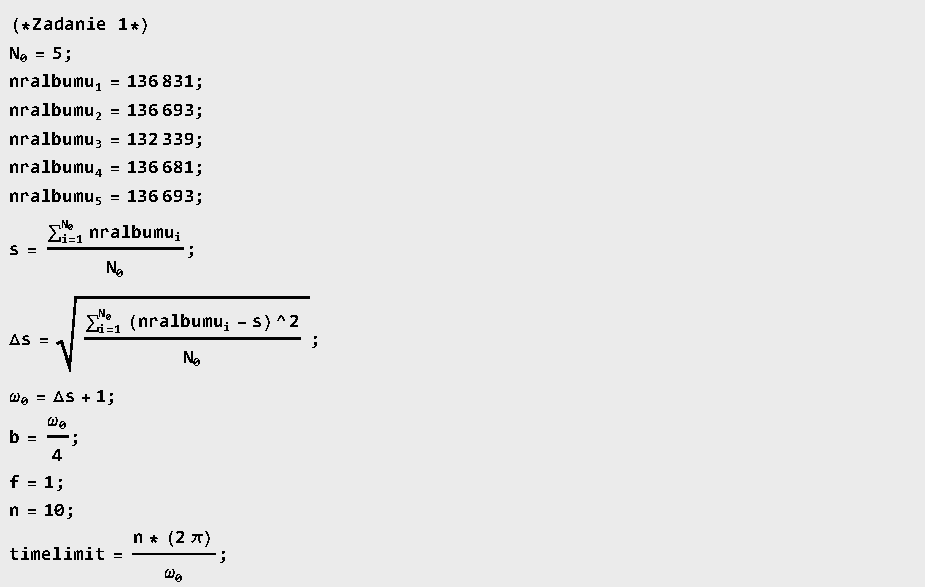
\includegraphics[scale=1]{zad1}
				\captionof*{fiure}{Zrzut ekranu kodu napisanego w programie {\em Mathematica} w celu wykonania zadania}
		\end{figure}

		\subsection{Przeprowadzenie rozwiązań numerycznych, oraz prezentacja ich wyników dla podpunktu $ a) $ $\omega = \sqrt{\omega_{0}^2 - \frac{1}{2}b^2}$}
		
				\begin{figure}[H]
			\centering
			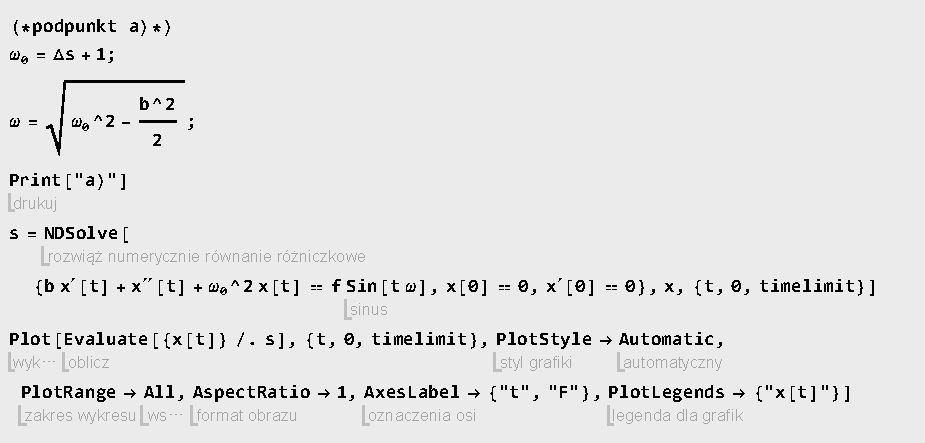
\includegraphics[scale=1]{1a}
			\captionof*{fiure}{Zrzut ekranu kodu napisanego w programie {\em Mathematica} w celu wykonania zadania}
		\end{figure}
	
		\subsubsection*{Prezentacja wyników dla podpunktu a}
		
						\begin{figure}[H]
			\centering
			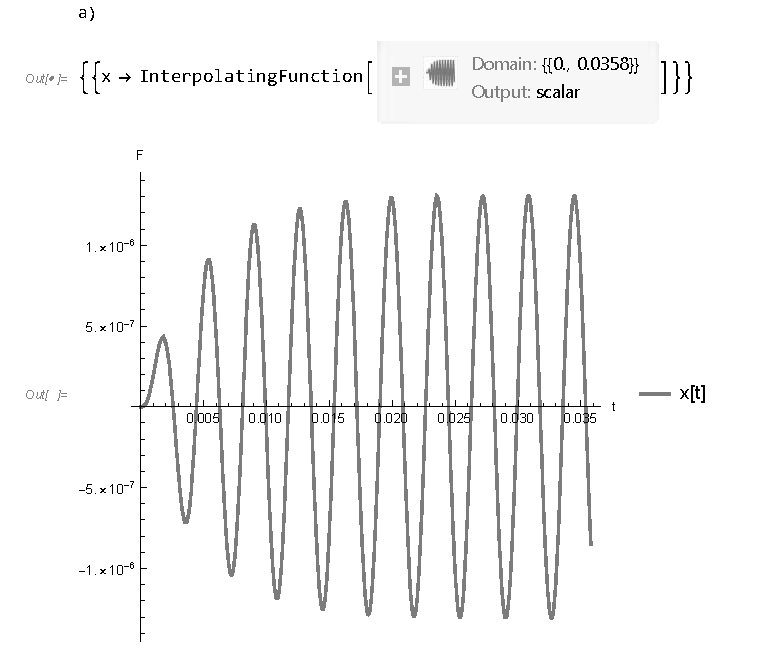
\includegraphics[scale=0.9]{wyk1}
			\captionof*{fiure}{Zrzut ekranu prezentujący wyniki wygenerowane przez program {\em Mathematica} dla podpunku a}
		\end{figure}
		
		\subsection{Przeprowadzenie rozwiązań numerycznych, oraz prezentacja ich wyników dla podpunktu $ b) $ $\omega = \frac{3}{4}\sqrt{\omega_{0}^2 - \frac{1}{2}b^2}$}
		
				\begin{figure}[H]
	\centering
	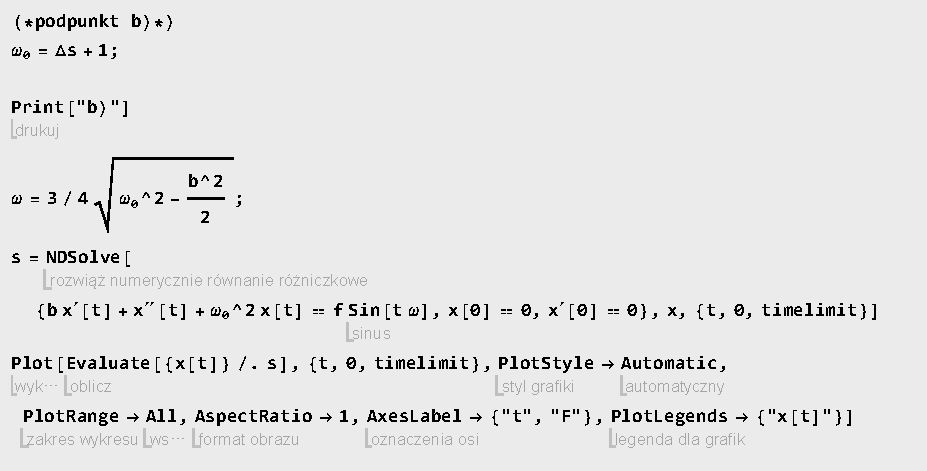
\includegraphics[scale=1]{zad1b}
	\captionof*{fiure}{Zrzut ekranu kodu napisanego w programie {\em Mathematica} w celu wykonania zadania}
\end{figure}
		
		\subsubsection*{Prezentacja wyników dla podpunktu b}
		
								\begin{figure}[H]
			\centering
			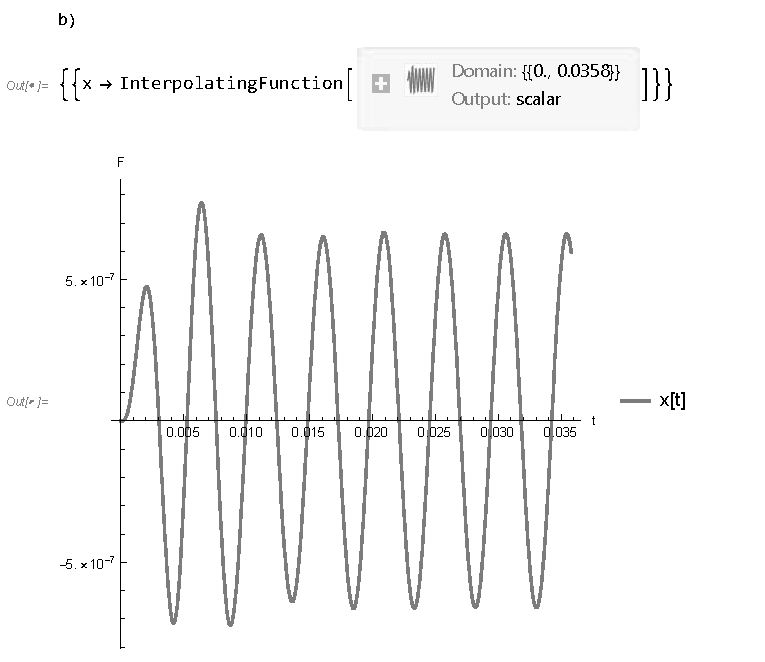
\includegraphics[scale=0.9]{wyk2}
			\captionof*{fiure}{Zrzut ekranu prezentujący wyniki wygenerowane przez program {\em Mathematica} dla podpunku b}
		\end{figure}
		
		\subsection{Przeprowadzenie rozwiązań numerycznych, oraz prezentacja ich wyników dla podpunktu $ c) $ $\omega = \frac{5}{4}\sqrt{\omega_{0}^2 - \frac{1}{2}b^2}$}
		
		
						\begin{figure}[H]
			\centering
			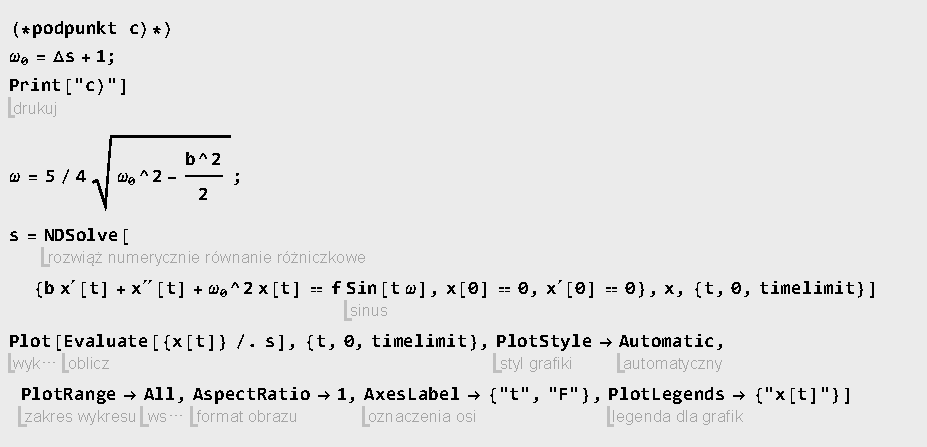
\includegraphics[scale=1]{1c}
			\captionof*{fiure}{Zrzut ekranu kodu napisanego w programie {\em Mathematica} w celu wykonania zadania}
		\end{figure}
		
		\subsubsection*{Prezentacja wyników dla podpunktu c}

		\begin{figure}[H]
			\centering
			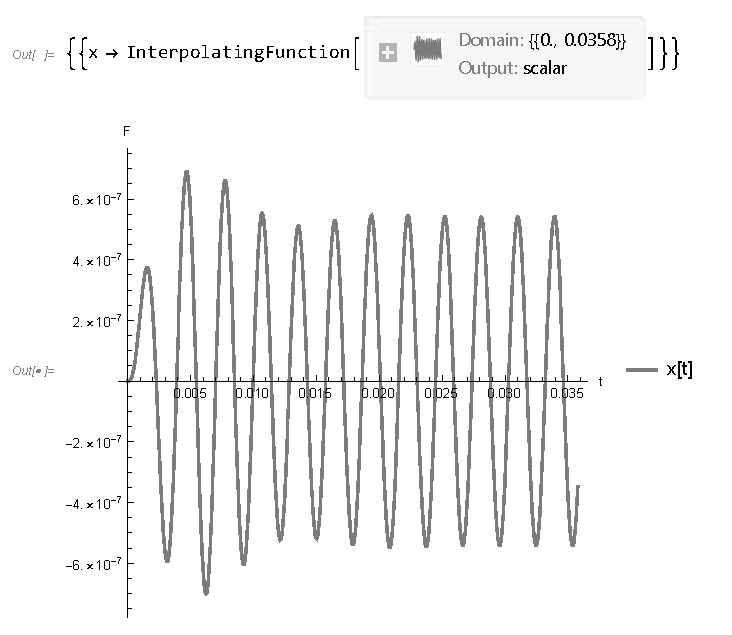
\includegraphics[scale=1]{wyk3}
			\captionof*{fiure}{Zrzut ekranu prezentujący wyniki wygenerowane przez program {\em Mathematica} dla podpunku c}
		\end{figure}
		
		\section{Generacja wykresu punktowego, oraz tabeli $X_{0}(\omega)$, zależności maksymalnej amplitudy drgań $X_{0}$ od częstotliwości $\omega$ przyjmując wartości $\omega_{k} = \frac{5}{4}\sqrt{\omega_{0}^2 - \frac{1}{2}b^2}$, gdzie $k = 1,2,\cdots,19;$}
		
						\begin{figure}[H]
			\centering
			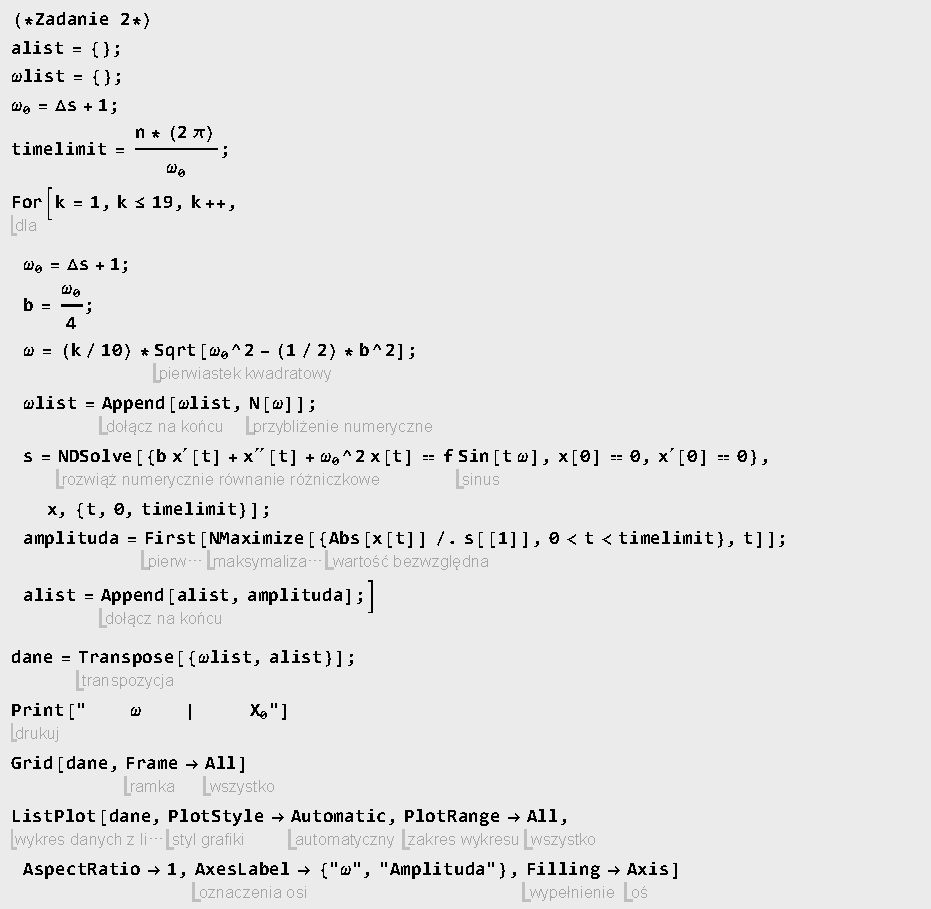
\includegraphics[scale=1]{zad2}
			\captionof*{fiure}{Zrzut ekranu kodu napisanego w programie {\em Mathematica} w celu wykonania zadania}
		\end{figure}
	
	
		\subsubsection*{Prezentacja wyników}
		
		\begin{figure}[H]
			\centering
			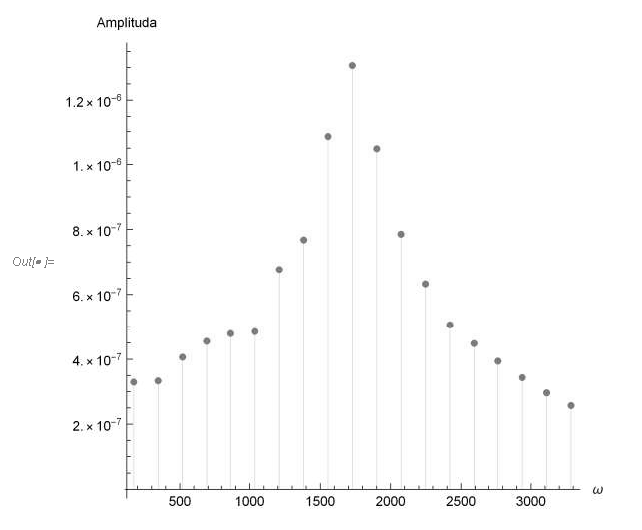
\includegraphics[scale=0.9]{wykpunkt}
			\captionof*{fiure}{Zrzut ekranu prezentujący wyniki wygenerowane przez program {\em Mathematica}}
		\end{figure}
	
		\begin{figure}[H]
	\centering
	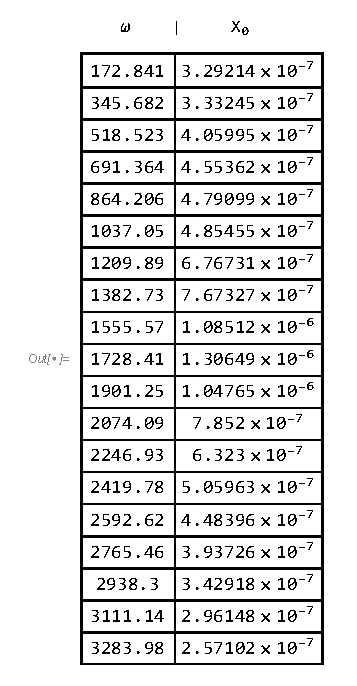
\includegraphics[scale=0.9]{tabela}
	\captionof*{fiure}{Zrzut ekranu prezentujący tabele wygenerowaną przez program {\em Mathematica}}
	\end{figure}
	
	
	\section{Obliczenie wartości $ \triangle \omega $}
	
	
							\begin{figure}[H]
		\centering
		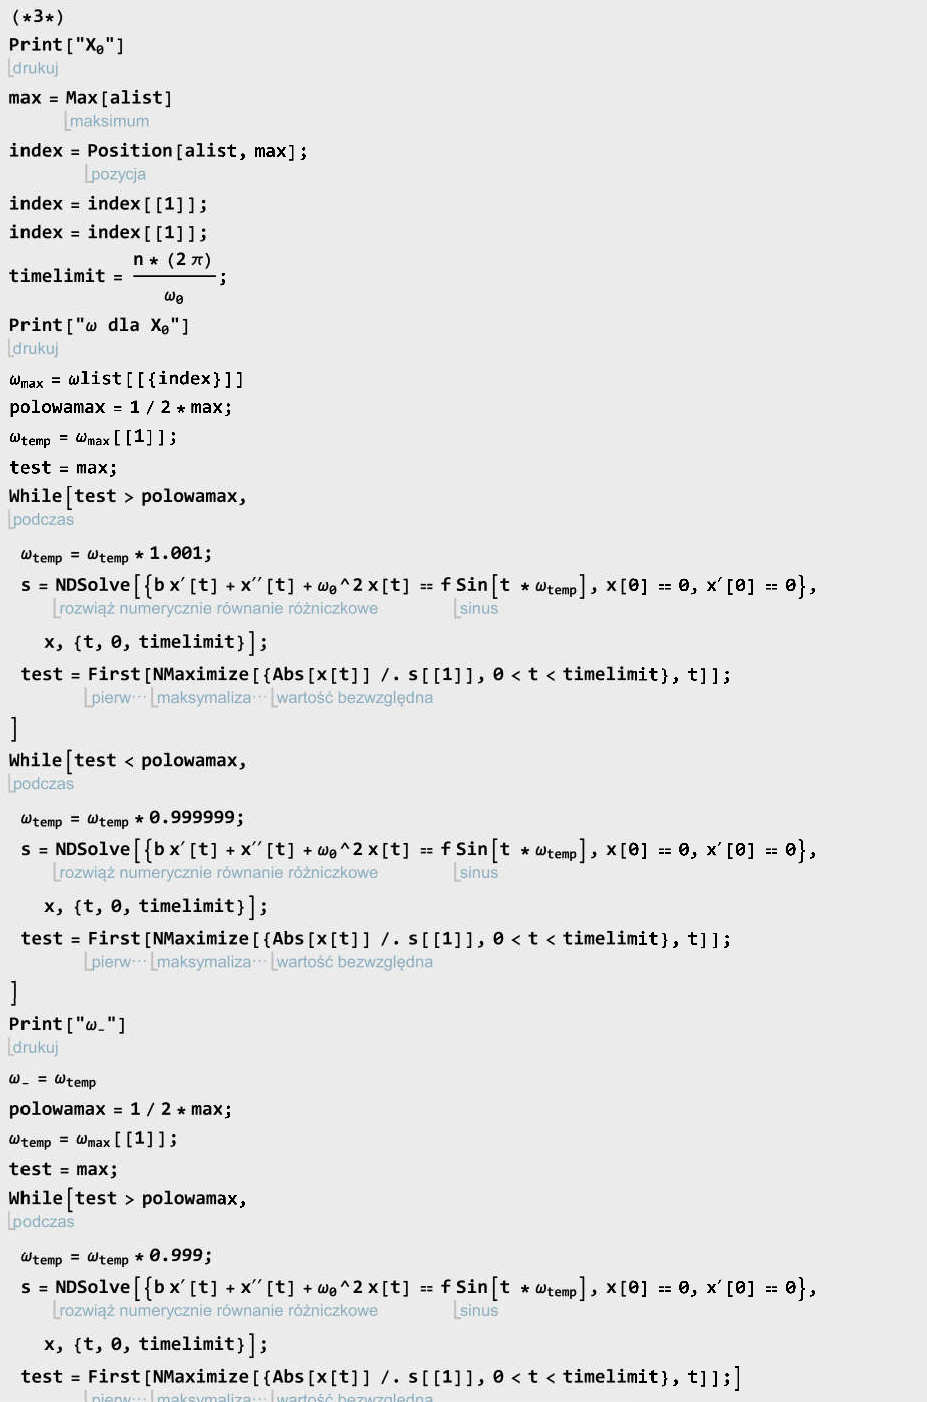
\includegraphics[scale=0.9]{zadanie3_1}
	\end{figure}

			\begin{figure}[H]
		\centering
		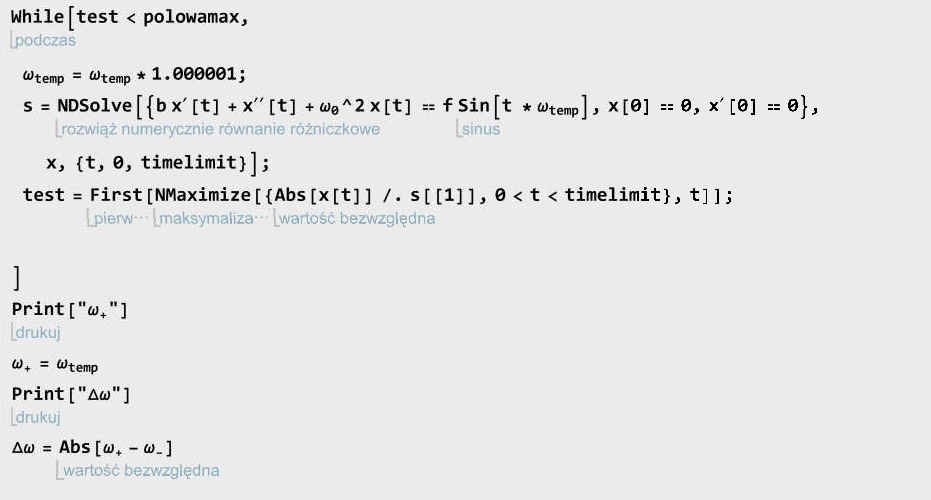
\includegraphics[scale=1]{zadanie3_2}
		\captionof*{fiure}{Zrzut ekranu kodu napisanego w programie {\em Mathematica} w celu wykonania zadania}
	\end{figure}
		\subsubsection*{Prezentacja wyników}

\begin{figure}[H]
	\centering
	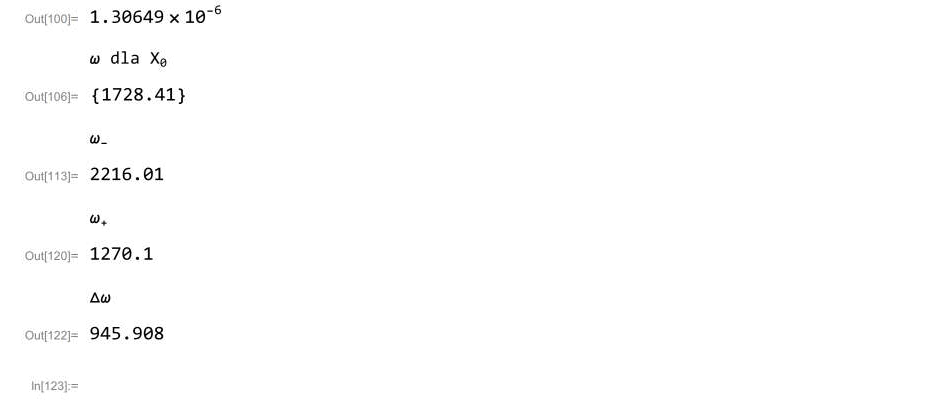
\includegraphics[scale=1]{zadanie3odpowiedz}
	\captionof*{fiure}{Zrzut ekranu prezentujący wyniki wygenerowane przez program {\em Mathematica}}
\end{figure}

	\newpage
	\tableofcontents

\end{document}


